\documentclass[a4paper]{article}
\usepackage{vub}

\usepackage{pgfplots}
\usepackage{hyperref}
\usepackage[font=small,labelfont=bf]{caption}
% Some highly suggested packages. Please read their manuals.
\usepackage{cleveref}
\usepackage[final]{pdfpages}
\usepackage[square, numbers]{natbib}
\usepackage{float}
\bibliographystyle{abbrvnat}

\newcommand{\dquote}[1]{``#1''}
\newcommand{\squote}[1]{`#1'}
\newcommand{\codes}[1]{\texttt{#1}}


\setlength{\parskip}{\baselineskip}%
\setlength{\parindent}{0pt}%

\title{Project Erlang}
\author{Silken Heynderickx}
\faculty{Science and Bio-Engineering Sciences}
\promotors{Prof. Dr. ???}
\pretitle{Multicore Report (task Erlang) submitted in partial fulfilment of the requirements for the degree of Bachelor of Science in de Computerwetenschappen}
\date{2023-2024}
\pgfplotsset{compat=1.18}

\begin{document}
\maketitle

\tableofcontents

\newpage

\section{Overview}

My first implementation was based on the first character of the user's username to put them in the server that has their initial (based on ANSII order). I did not use this implementation because, first of all, when a new user was added, and the dictionary had more users than the threshold, the range of ANSI characters was split into 2, and the users were moved to the other server. This means that when a user made a new request but was replaced, we needed to keep track of the replaced users to send them to their new server, so every request would need to be used to send to the correct server. Second, when the range of ANSII characters is split into 2, most of the usernames still fall under the same new range, which causes the new server to be empty and the old one to be full. Third, you had to update all existing servers to where the users were placed or that servers needed to go over different servers (depending on where splitting happened) to find the newly created server. This would cause a chain of requests to different servers. Nothing unsolvable, but there were more accessible and more performant ways to make this implementation work. 
(This implementation is saved under server\_parallelized.erl) 

The implementation I used for the experiments is based on one server that makes other servers where users can send requests, too. When a user is registered, a new server will be assigned. This does not cause a bottleneck because it only handles register requests or sometimes redirects requests to another server (ex., when the following user is called). That server holds an ordered dictionary of the usernames with their server saved. A new server is created to save new users whenever a server is full (depending on the threshold). Each server has its own users with their data. When a particular user sends a message, the followers will get that message saved in their timeline (this causes data to be saved on multiple servers). I have chosen a more performant solution for the timeline instead of lower memory usage and no duplicated data. When a user follows a new user, the server of the following user will be saved to the server that requested the PID. So, PID will also be saved in different places simultaneously, but this has the advantage that the initial server will not have "too much" of a bottleneck to redirect messages. 

For the experiments, our focus was on three key performance metrics: Speedup, Latency and throughput, and Broadcasting a message. 


\section{Implementation}

\subsection{Architecture}

\begin{figure}[H]
	\centering
	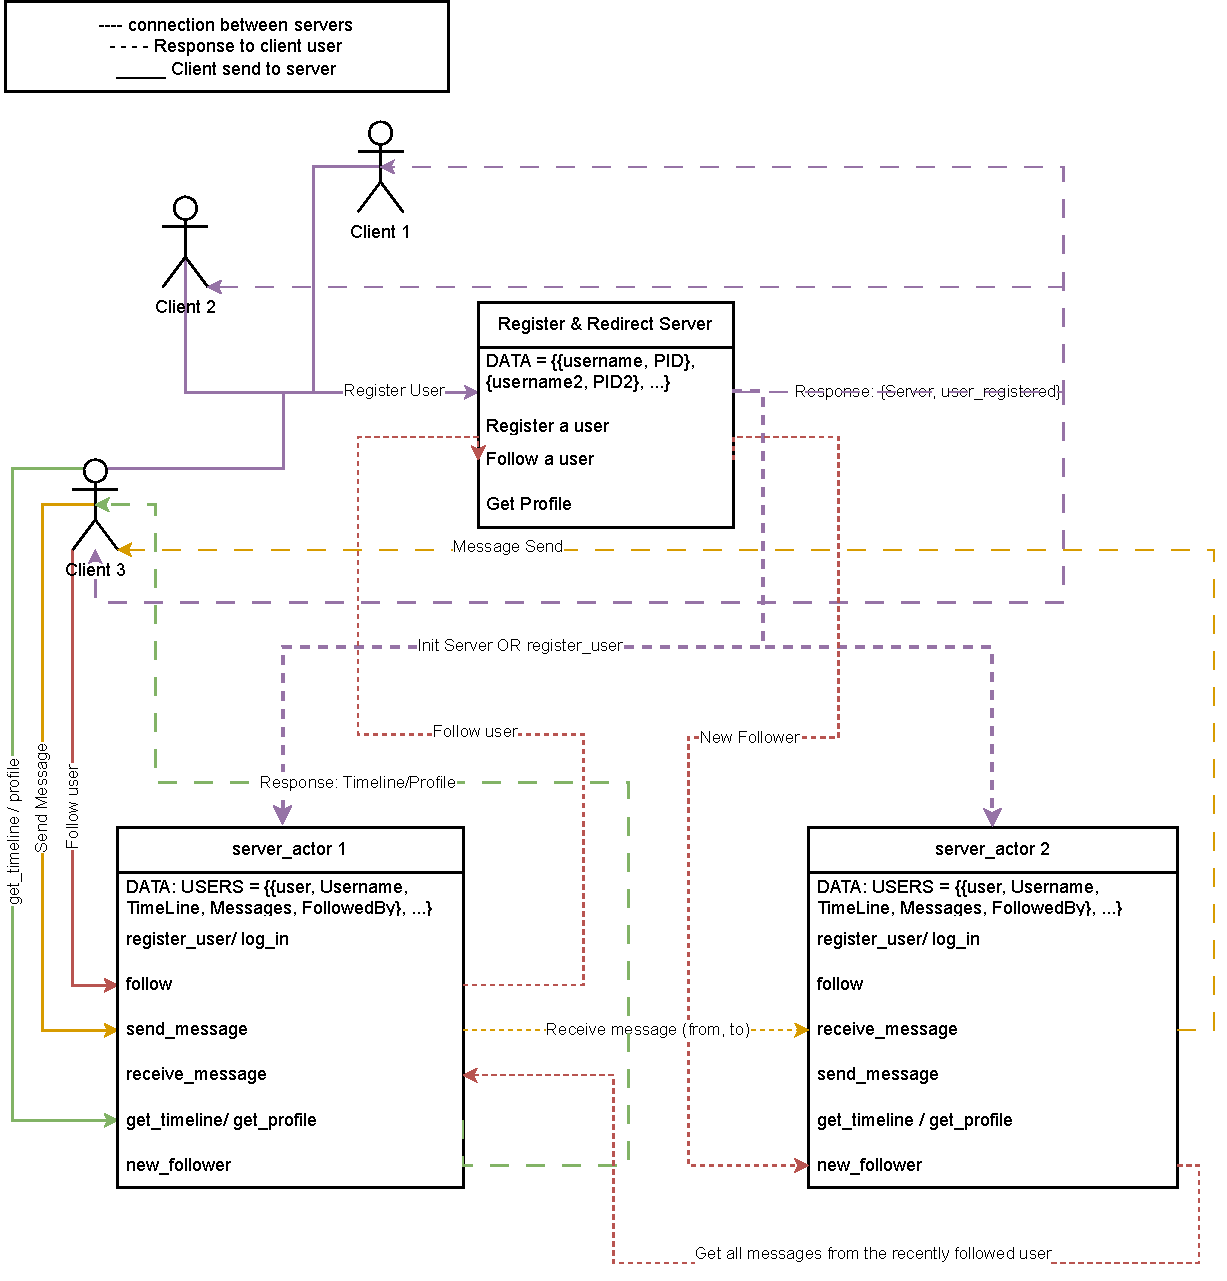
\includegraphics[width = \linewidth]{Architecture.pdf}
	\caption{
		This flowchart gives an overview of the architecture, how messages flow between the actors, and where which data is stored. (Every color of the lines, are new requests from the client and the path it follows)
	}
\end{figure}

For the case of showing the architecture, I made three clients, and these all send the Register User to the ''Register \& Redirect Server''; then adds the user to an existing server\_actor or makes a new server\_actor depending on the threshold (amount of users per actor).
It sends then the \{PID, user\_registered\} back to the client. When the client receives this message, it can send a new request to that server. 

With "the client," I wanted to display four different requests a user can send: "get\_timeline, get\_profile, send\_message, follow."
Get\_timeline and get\_profile, in this case, the user asks for its timeline or profile; the timeline is saved in the actor the user sends to.
So the server will send a response directly to the user with the timeline.
If the user is not part of the current actor, it will send the "Register \& Redirect" to redirect the message to the correct actor.
This can cause a bottleneck when having many register/ follow and get\_profile requests.
This can be solved by saving the actor ID of users in every server\_actor, but when having lots of users, this would cause a lot of data duplication.
I choose to have data duplication to save the messages instead of user\_pids.
From my experience, when we scroll, we mostly look at the timeline and maybe view a few other profiles.
So, I choose to make "get\_timeline" as performant as possible. 

When a user sends a new message, it will send the message to every follower of that user and save it in their timeline. (What we also could have done here to avoid data duplication but keep the timeline as performant as possible is only saving the X most recent messages, and when a user scrolls further than those, the server will need to fetch them. Nevertheless, this was out of this project's scope because we could not know when a user would look at all the timeline messages). When getting new messages, they are inserted in an orddict that is already sorted from new to old, so we do not need a sorting algorithm when get\_timeline is called.

When a user follows another user, the PID will be requested to the Register \& Redirect server, and the follower will also be sent to the following user. 
Requesting the PID of the following user will not cause a deadlock because the server\_actor does not wait for a response but saves the PID by the correct follower. This can cause some inconsistency in the follower's data, but often, when scrolling online, the timeline does not get refreshed every time you follow a new user, so this will not cause an issue. 

%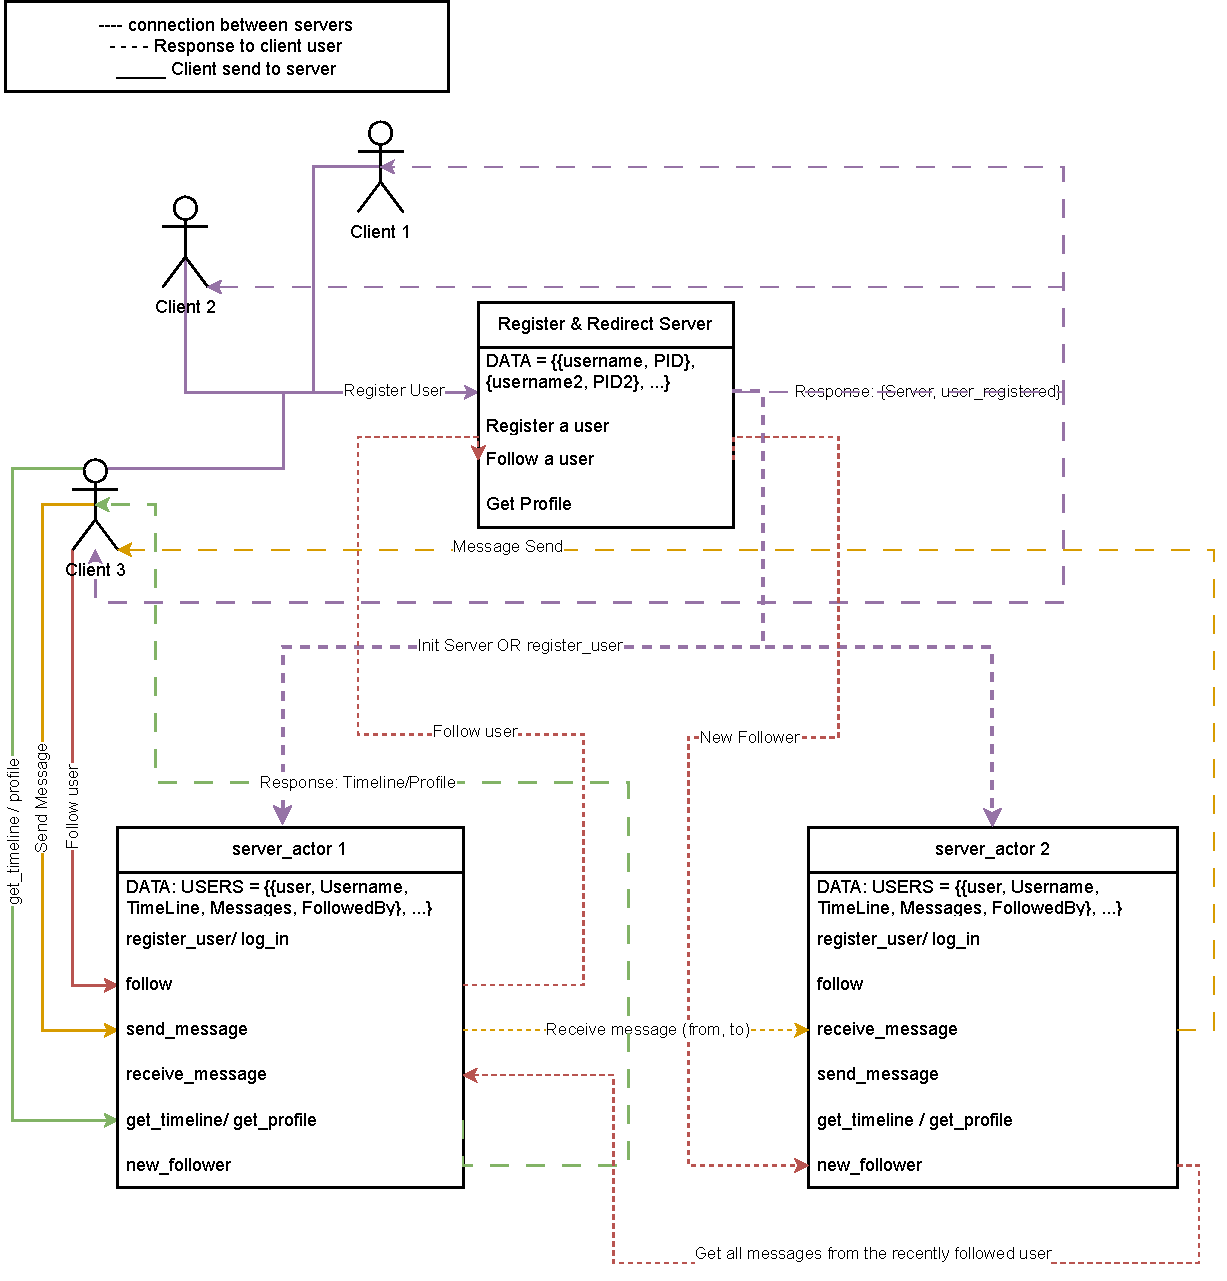
\includepdf[pages=-]{Architecture.pdf}

\subsection{Scalability}

\subsubsection{How does your design ensure scalability? What is the best case and the worst case in
terms of the mix of different user requests? When would the responsiveness decrease?}
The best case of my implementation would be when the requests are a mix of requests, with a preference for timeline requests and sending messages; this would typically not cause any decrease in responsiveness. However, when there is an overload of register\_user, follow and get\_profile requests, the Register and redirect server would get a bottleneck. As explained before, I focussed on the timeline to be as performant as possible. In real life, this is the most sent request; every time you open an app, this request will automatically be sent.

In most cases, there will not be a chain of register\_user and get\_profile. Sometimes, follow bots are made for users to farm followers, which would cause a big issue for our app's responsiveness. \subsubsection{How do you ensure conceptual scalability to hundreds, thousands, or millions of users?
Are there any conceptual bottlenecks left?}

The application is very scalable when you choose how many users will be handled per actor. Because of the benchmarks I tried on my local computer, one user/ server performs the best when there are 100 to 1000 users. However, when we have an app, of course, we want the app to succeed with the goal of millions of users. When there are millions of users, the changes are so significant that the Register and redirect form a bottleneck to the system. This could be resolved by splitting that server into multiple servers that handle different users' requests depending on which server they need to contact. Nevertheless, when we talk about millions of users, the server could also be distributed worldwide so that the users could send it to a server depending on their location. When we talk about millions of users, we will use parallelism and distributed systems, which would give us more possibilities to work with.

\subsubsection{ Where did you sacrifice data consistency to improve scalability? How does this decision improve scalability? In which case would the overall data consistency suffer most? }
When you follow a new user and then ask for the timeline, the user doesn't know which server to connect to for the new follower's messages. This would not cause a big issue because your timeline does not refresh when you follow a new user. This improves scalability because the server doesn't need to wait for the ID of the follower's server, so new requests can already be sent to the server. 

\section{Evaluation}
\subsection{Experimental set-up}
\subsubsection{Which CPU, tools, platform, versions of software, etc. you used }
\textbf{Firefly} \\
CPU: AMD Ryzen Threadripper 3990X Processor (64 core / 128 Threads, at 2.9 GHz base, 4.3 GHz boost) \\
RAM: 12 GB (DDR4 3200 MHz) \\
OS: Ubuntu 20.04.5 (Linux kernel 5.4.0-137-generic) \\
Erlang/OTP version: 22.2.7 \\

\textbf{Local PC:} \\
CPU: 10 cores (6 performance, 4 efficientie) Apple M2 Pro \\
RAM: 16 GB (LPDDR5 Hynix) \\
OS: macOS 14.2.1 (macOS Sonoma) \\
Erlang/OTP version: 26.2.3 \\

\subsubsection{ All details that are necessary to put the results into context.}
When doing benchmarks you need to know that there will always be programs that still use some performance of the CPU. But this should not have a big impact on the benchmarks. Although on the firefly I also noticed, that I was not alone that was executing tasks, this could have impacted some of my benchmarks. This is also why I choose to use the benchmarks on my local computer too for analyses and forming conclusions.
\subsubsection{All the parameters that influenced the run-time behavior of Erlang.}
I haven't changed anything from the erlang parameters (ex heap-size, ....). Those setting stayed on default. Before every benchmark I stopped all actors, before going into a new benchmark. So the actors wouldn't cause any interferance between benchmarks. Setting up the actors took the most time for the benchmarks (because of the register bottleneck).

\subsection{Experimental methodology}
! In the figures, 
I also tested the benchmarks on my local computer but did not delete the data tested for more threads than my computer had. I do not consider this data when forming my results when looking at the figures. The data should mostly be consistent and have no improvement from 10 cores and above.

I also used the runs from the benchmarks of my computer because setting up the benchmarks is sequential. Because of this, my PC significantly outperformed the Firefly in time of all benchmarks combined. The benchmark on my PC took around 5 hours, which would be sufficient to test on Firefly, but I didn't know that the sequential setup would influence the runtime on the Firefly so extensively. So on Firefly, I could only test for 1, 2, 4, 8 and 64 threads. I intended to test for 1, 2, 4, 8, 16, 32, 64 and 128 threads. I thus needed my local benchmark to better analyse the benchmarks.   

\subsubsection{How did you measure? E.g. using wall clock time or CPU time on the client side or server side.}
I measured using wall clock time when sending multiple requests simultaneously because, with CPU time, we only calculate the computed time of a unit. However, it is also important to keep track of a task when it is in a waiting state, which the CPU time does not.
Without keeping track of the waiting time, it would be like measuring the acceleration of an object without taking friction into account.
I measured on the client side, because we want to know when a client gets a response back from the server, or when the client can actually see the adjustments they made.
\subsubsection{How often did you repeat your experiments, and how did you evaluate the results?}
I repeated every experiments 30 times because how more you perform the experiments, how more accurate your results are. But because we only had a limited time on the firefly, I choose to execute multiple test cases, rather have only a few with more "certain" data. 30 times are in most case suffecient enough to get a good overview of the benchmarks.
I also discarded the first five experiment runs to take into account potential warmup time.

\subsection{Three experiments}
\subsubsection{What (dependent) variable(s) did you measure? For example: speedup, latency, 
		throughput, degree of inconsistency.}
		Experiment 1: Speedup \\
		Experiment 2: Latency \& throughput \\
		Experiment 3: Broadcasting \\
\subsubsection{What (independent) parameter did you vary? For example, number of scheduler threads,
number of server processes, users, messages, followers, number of simultaneous requests }
		Experiment 1:		
		\begin{itemize}
			\item Users/server process (number of server processes)
			\item  Amount of subscriptions 
			\item  Amount of users
		\end{itemize}
		Experiment 2:
		\begin{itemize}
			\item Amount of simultaneous requests (get profile)
			\item Amount of threads 
		\end{itemize}
		Experiment 3:
		\begin{itemize}
			\item Amount of followers when sending a message
			\item Amount of threads
		\end{itemize}

\subsubsection{Describe the load that you generated and other relevant parameters. What are the pro-
portions of different requests? How many users/messages/followers per user does your
system contain, how many clients are connected simultaneously, and how many requests
are there per connection?}
        	Experiment 1:
		To test the speedup of Users/ server I have following parameters
		\begin{itemize}
			\item  1000 Users / Server, 500 Users / Server, 100 Users / Server, 10 Users / Server, 1 User / Server 
			\item  1000 simultaneous users that are connected
			\item  25 subscriptions per user (be carefull, this doesn't mean that every user has 25 followers!)
			\item  10 messages per user
		\end{itemize}
		To test the speedup of requests depending on the amount of threads.
		\begin{itemize}
			\item For each kind of request 5000 users, 25 subscriptions, 10 messages / user
			\item Duration requests 1 Thread / n Threads
			\item Duration request SEQ implementation / n Threads Parallel implementation 
		\end{itemize}

		Experiment 2:
		To test the latency, I requested for every user its profile
		\begin{itemize}
			\item latency: requesting your profile, send 1 message  
			\item Throughput: 10000 times requesting your profile (different users), send 10000 messages, 10000 get timeline requests 
		\end{itemize}
		Experiment 3:
		\begin{itemize}
			\item 1 user per actor, 5000 users, 10 messages, X amount of followers (amount of followers tells us how many servers we need to contact), sending 1 message  
			\item How long it takes to send to multiple servers (No other server, 10 other servers, 20 other servers and 50 other servers on M2 pro ship), when send to the server the user will see it in their timeline.
			\item How long it takes to send to multiple servers (No other server, 10 other servers on Firefly), when send to the server the user will see it in their timeline. 
			\item Amount of Threads: 1, 2, 4, 8, 16, 32 (M2 pro); 1, 2, 4, 8, 64 (Firefly)
		\end{itemize}


\subsubsection{Results Experiment 1}
\begin{figure}[H]
	\centering
	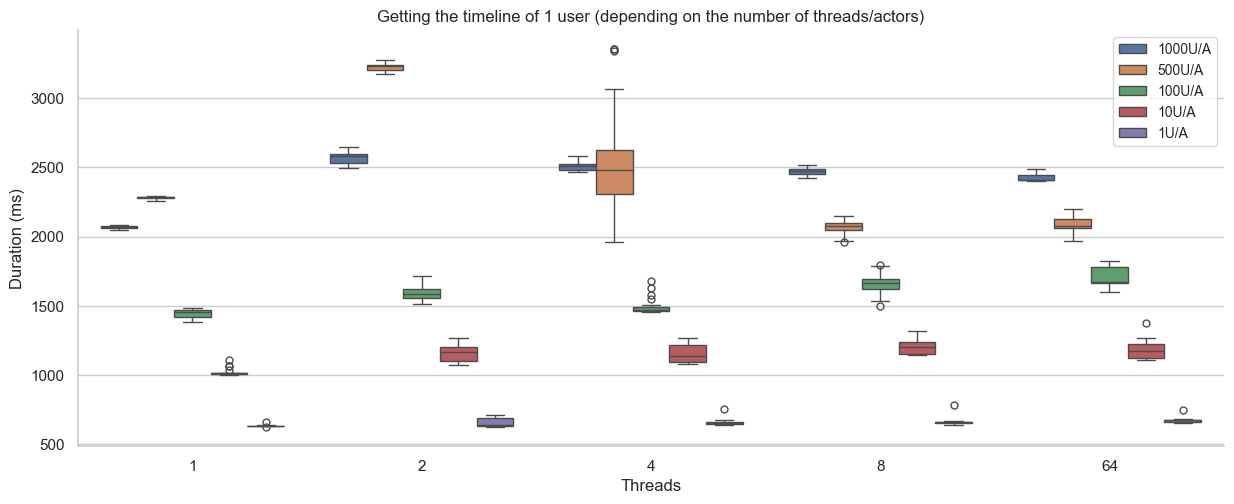
\includegraphics[width = \linewidth]{Images/Speedup(U:A)Box.png}
	\caption{Boxplots of amount of users per actor, while requesting the timeline of a user}
\end{figure}
In this figure, we can already see that the duration to get the timeline of 1 user per actor is significantly faster than when we have more users per actor. When we have 500 Users / Actor the data is somewhat unexpected, it is not really constant depending on the amount of threads. I don't have a certain explanation for why this happened, but what I think happened is that there were other processes running on the Firefly server. I noticed that there was someone else on the server and a process that a user forgot to close (but this didn't take much CPU usage and was constant throughout the whole benchmark when I looked at it). But this could be an explanation.

\begin{figure}[H]
	\centering
	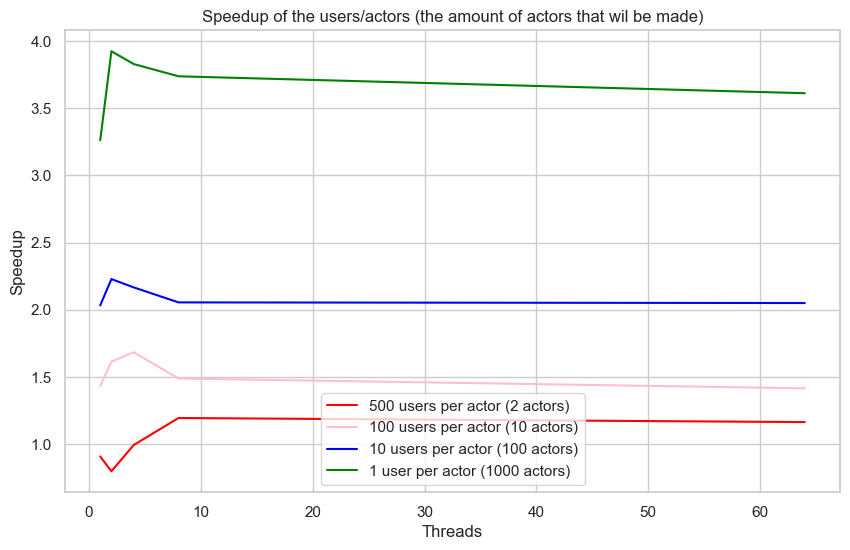
\includegraphics[width = \linewidth]{Images/Speedup(U:A).png}
	\caption{Speedup of the amount of users per actor}
\end{figure}
I chose not to display the inconsistent data of 500 users / actor in the speedup because it made the graph very unclear, but that doesn't mean that we should just forget about it. It is still important to keep in mind, we could find some data that can explain the previous results. Here we can cleary see that we have a speedup of around 3.5 when having 1 user / actor, compared to 1000 users / actor. I took 1000 user per actor as a reference for the speedup because for this testcase, it would mean that all users are on one actor. I choose to get the timeline of a user as reference of the number of users / actor, because there are not many other factors we need to keep in mind (ex sending to other servers, waiting for responses, ...). The speedup can be explained by the change in size of the ordered dictionary where we need to look up the user. We can also see a speedup from 1 to 8 threads. This can be explained because we still have the benefit that the scheduler does not need to do too much work to separate the tasks over the different threads. When the treads go to 64, it is already a huge amount of work for the scheduler to separate all the tasks among them. But to have a more extensive overview of the speedup separated over the number of threads, we did some other tests. This will be discussed later.  

\begin{figure}[H]
	\centering
	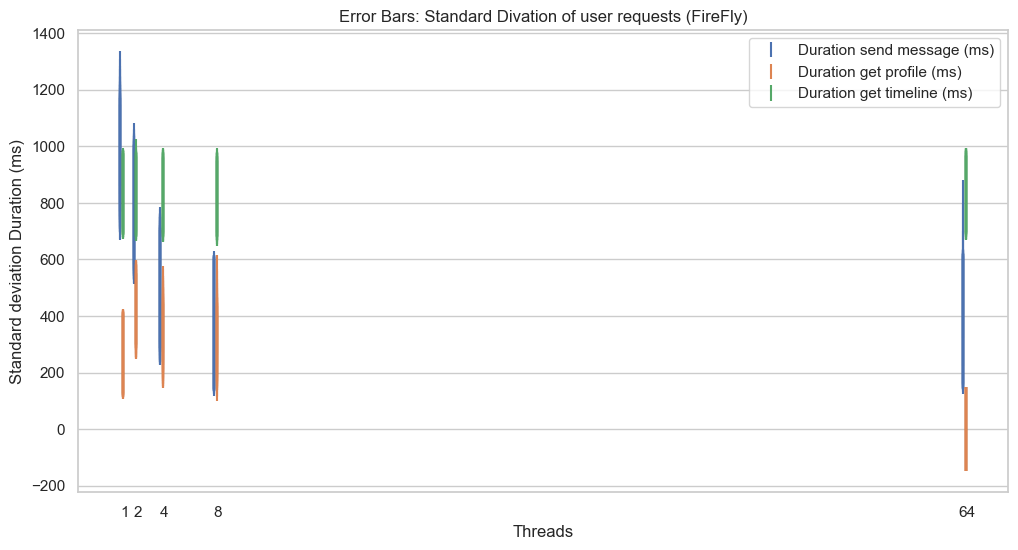
\includegraphics[width = \linewidth]{Images/SpeedupStdURFirefly.png}
	\caption{}
\end{figure}
\begin{figure}[H]
	\centering
	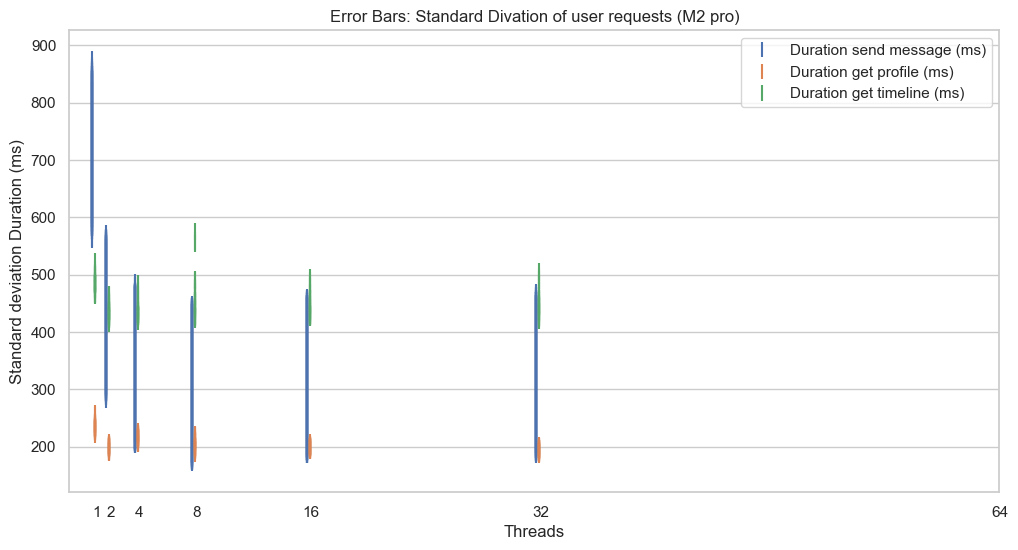
\includegraphics[width = \linewidth]{Images/SpeedupStdUR.png}
	\caption{}
\end{figure}
We can see here that the standard deviation of sending a message is the biggest of all.
This is what I expected to happen.
This is explainable because the number of followers (the number of actors to contact) is not constant. We know that every user follows 25 other users, but that does not mean that every user has 25 followers. The error range of get profile and get timeline are similar, this can be explained because get timeline and profile are both lookups in the same size of ordered dictionary. Get timeline seems to be slightly bigger than get profile, I think this is because the data to fetch in get timeline is more than the one in get profile. We can also conclude that the range of error is bigger on Firefly than the one on the M2 chip. This is not necessarily a bad thing, because we can see that every task also takes more time in proportion, this can be reflected in the error rate. Although the proportion of the error rate looks bigger than the time difference at first glance. This can be explained by the single core performance of the M2 chip that overpowers the one from the Threadripper.   

\begin{figure}[H]
	\centering
	\includegraphics[width = \linewidth]{Images/SpeedupURMeanFireflyCom.png}
	\caption{}
\end{figure}
We cannot really conclude where the Firefly exactly needs more time to schedule the tasks to different threads because of the lack of data from the Firefly benchmarks. But hypothetically we could see this when the duration doesn't really go down anymore or even goes back up a little. Get profile has a shorter line than the others because my timeslot ended when I started at 16 threads for get profile. When comparing get profile on the M2 chip, we get more explainable results, so for get profile I will focus more on the results of the M2 chip than the one on the firefly. 
\begin{figure}[H]
	\centering
	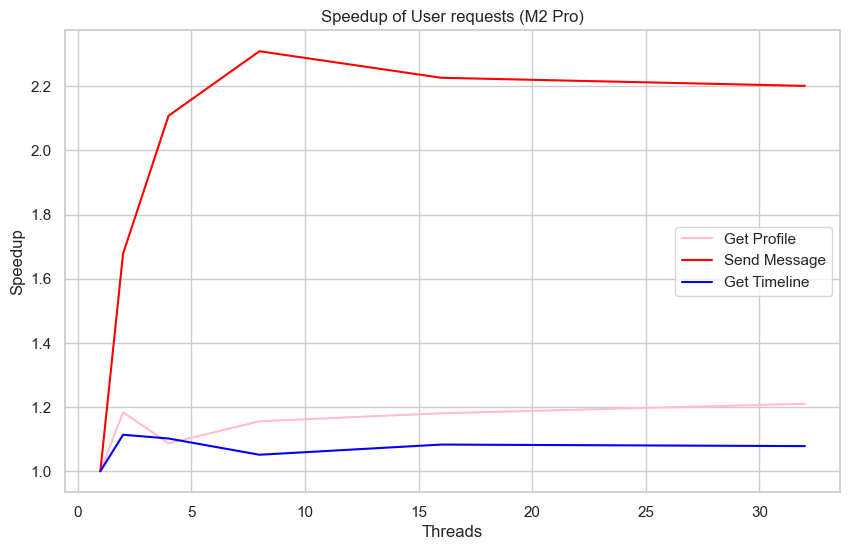
\includegraphics[width = \linewidth]{Images/SpeedupURMeanCom.png}
	\caption{}
\end{figure}
Here, we can clearly see that there is a huge speedup when sending a message. Send message contacts a lot of different actors, it can easily be done in parallel, this reflects on the speedup of Send message for the different amount of threads (this can also be seen on the same figure of the firefly). We should look more in detail get profile and get timeline to see if there is a speedup. But we can now also see that there is a speedup for "get timeline" and "get profile" too. The speedup is also best when we use 2 threads. This can be explained because the sheduler on the M2 needs more time after 2 threads, this doesn't say anything about the results on Firefly because the Multicore performance (so this also concludes the sheduler) should be better on the Firefly than on my computer. 
\begin{figure}[H]
	\centering
	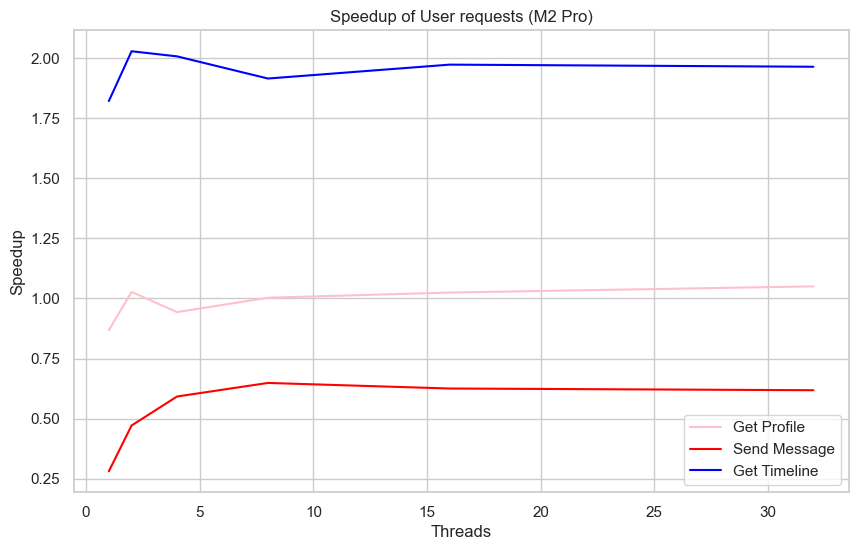
\includegraphics[width = \linewidth]{Images/SpeedupSeq.png}
	\caption{Speedup Sequential compared to Parallel implementation}
\end{figure}
We can see that the parallel implementation, compared to the Sequential implementation, has a 2x speedup. This is because I really valued the implementation of get timeline, because in my experience this would be the request that would happen the most, often in social media apps this will refresh in several time intervals whereas send message and new follower will only be send by the client. Also, most followers only sometimes post something or follow a few other users. Send message became slower, this is because it needs to contact a lot of different servers. But this has the best speedup. This only involved a lookup and a store in dictionary in the sequential implementation. With the parallel implementation we are using ordered dictionaries to make the lookup faster (which is an advantage for timeline, get profile) but this also means that the store is much slower. When we look at get profile, this stays somewhat the same than the sequential implementation.   

This is not everything for the speedup, in later experiments we will somethimes talk more about the speedup and have new findings. 

\subsubsection{Results Experiment 2}
\begin{figure}[H]
	\centering
	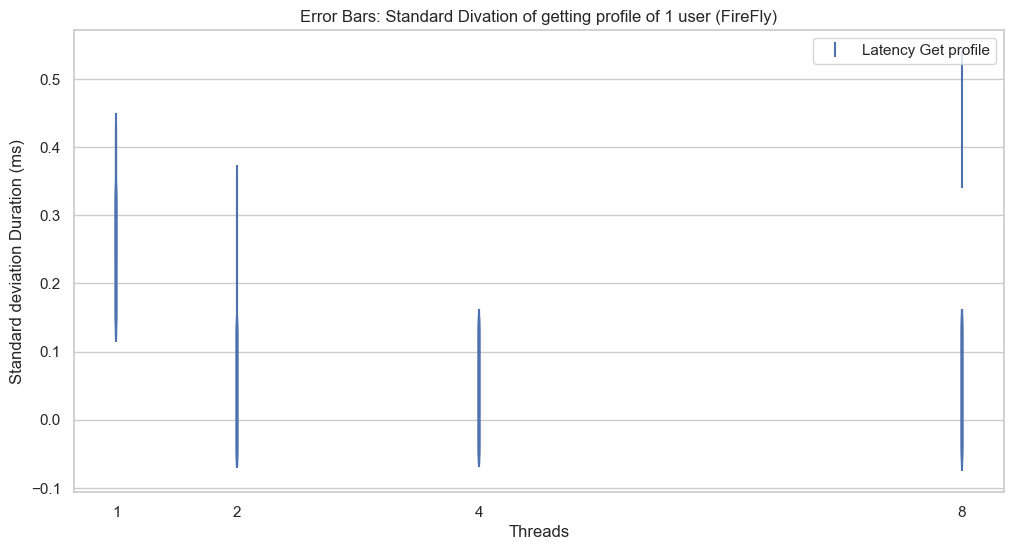
\includegraphics[width = \linewidth]{Images/LatencyStdFirefly.png}
	\caption{}
\end{figure}
The latency of a get profile request is the most stable when we use 4 threads (this is not necessarily the best result because of the lack of data). 
\begin{figure}[H]
	\centering
	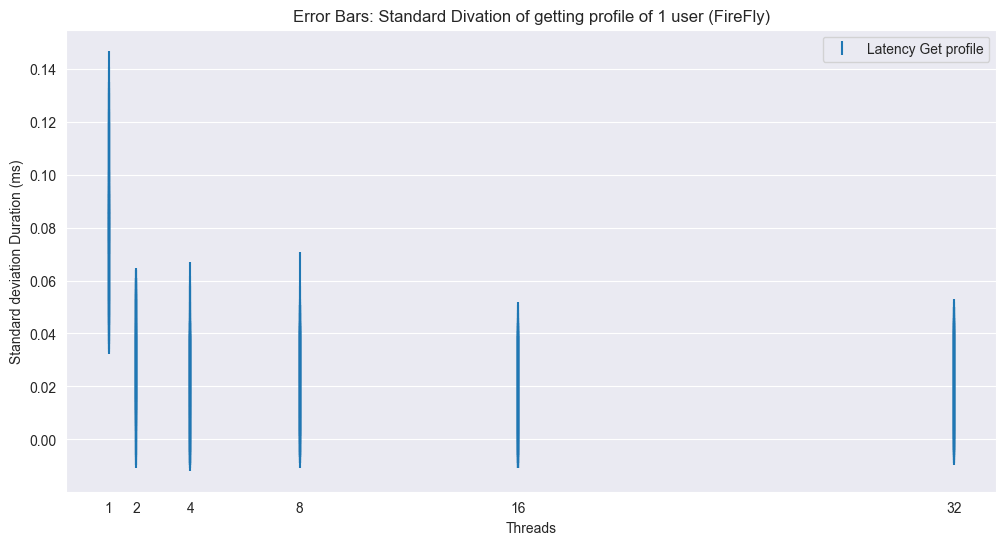
\includegraphics[width = \linewidth]{Images/LatencyStd.png}
	\caption{}
\end{figure}
We can see that the error rate of 1 thread is higher than using multiple threads. Because getting a profile takes less time when it can be executed in parallel than when you execute it with only 1 thread. Because it takes less time, the error rate will most likely also scale. 
\begin{figure}[H]
	\centering
	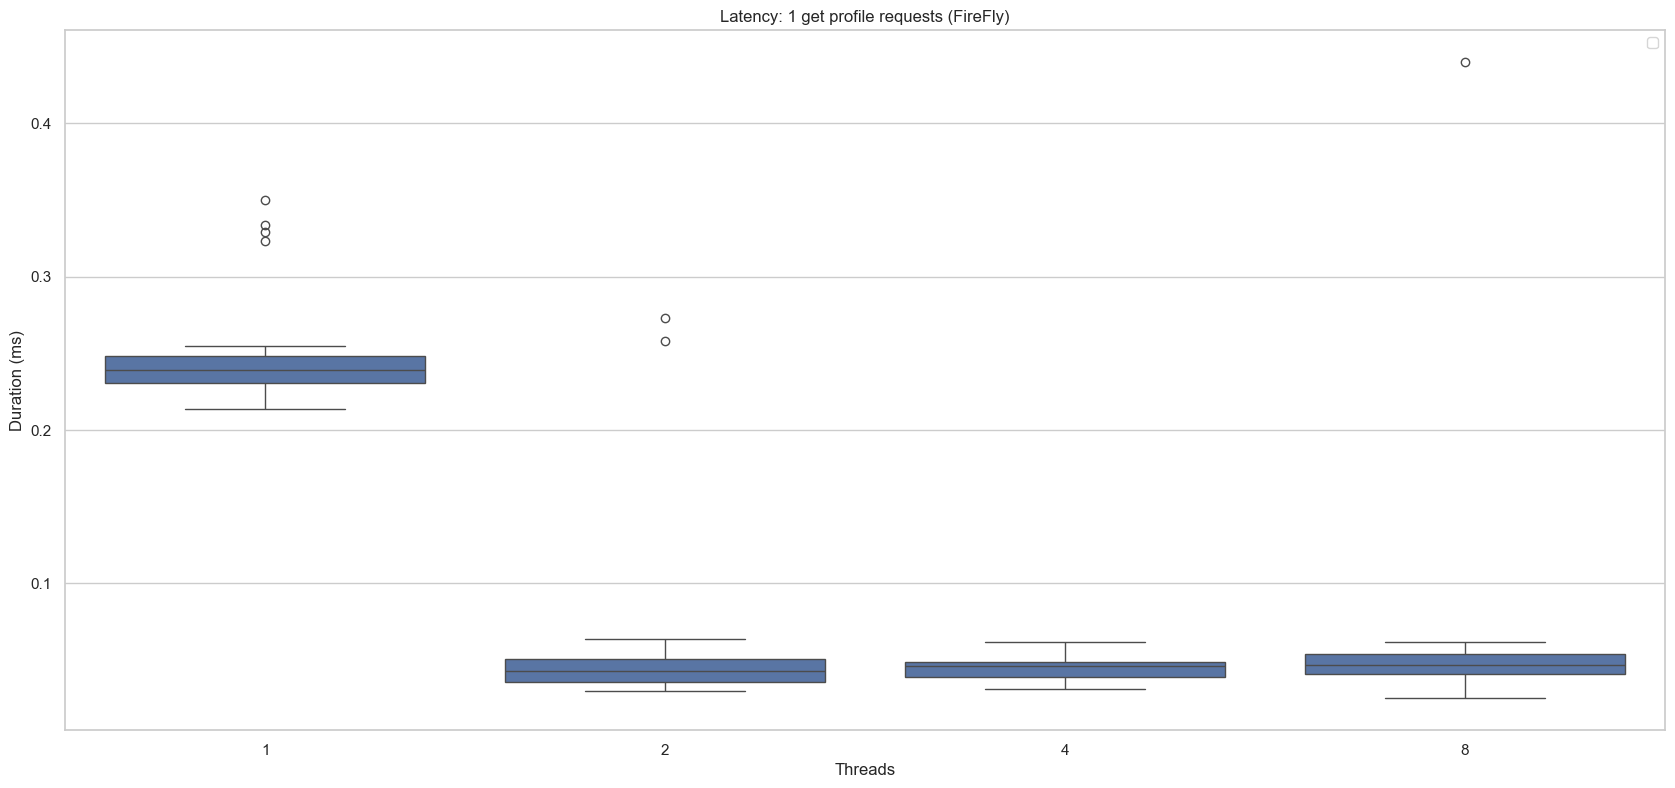
\includegraphics[width = \linewidth]{Images/LatencyBoxFirefly.png}
	\caption{}
\end{figure}
\begin{figure}[H]
	\centering
	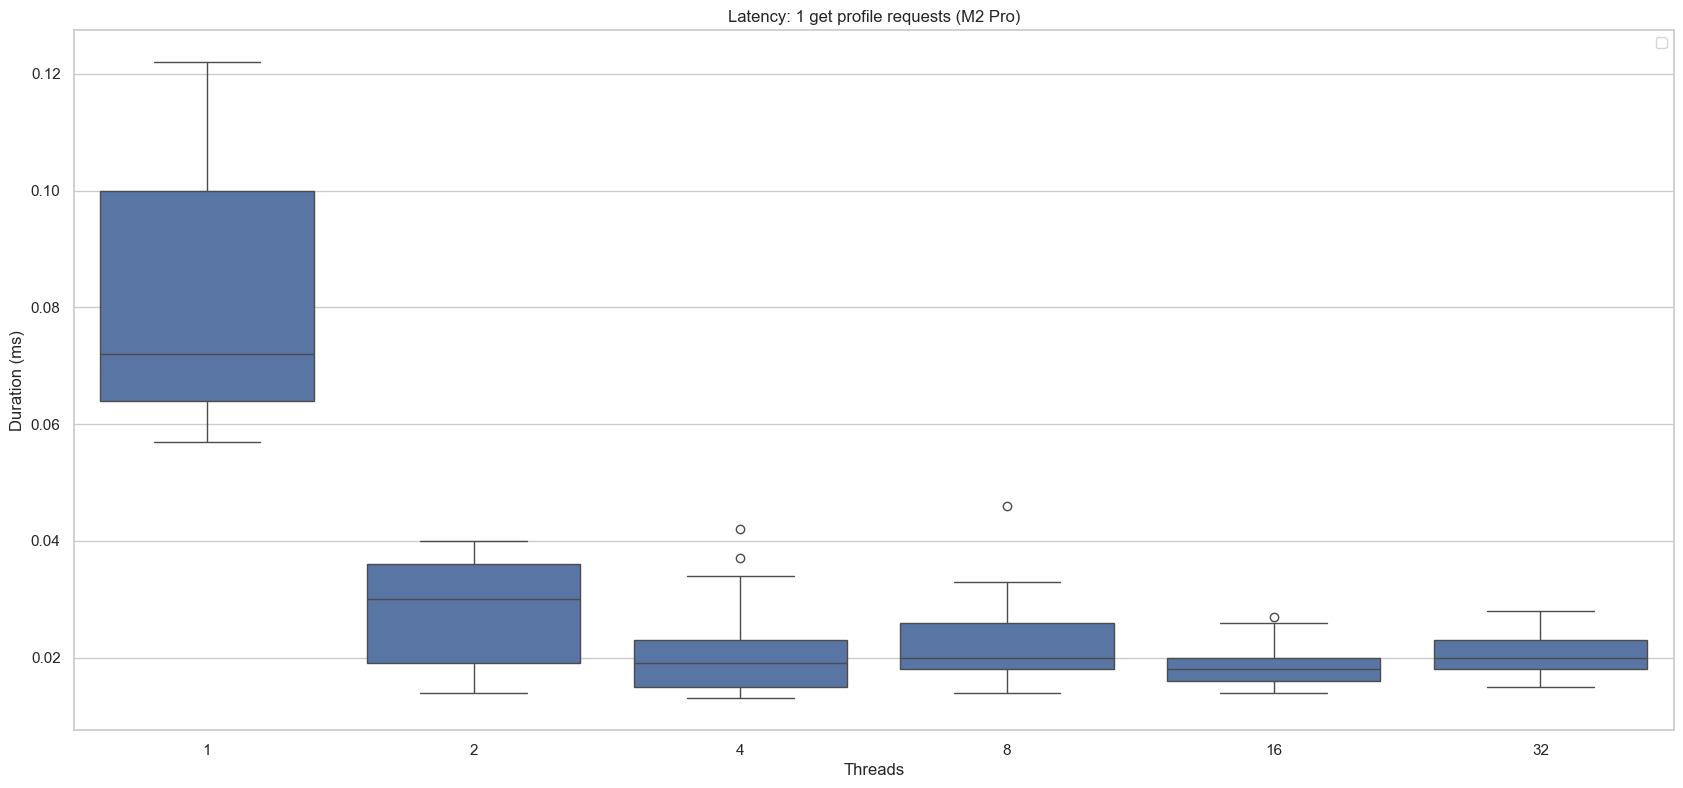
\includegraphics[width = \linewidth]{Images/LatencyBox.png}
	\caption{}
\end{figure}
Be carefull, the heigth of the boxes doesn't necessary differ from Firefly compared to the M2 chip, because the scale is different. Here we can see that getting a profile takes less time when having multiple threads active at the same time. This means that get profile has a speedup, compared to 1 thread. On the figure of the M2 chip we can also see that the data gets more concentrated when using more threads. The data is more stable, because there is more change that the get profile we request is on a different one than the previous. This could also be seen in the standard divation figure above.  
\begin{figure}[H]
	\centering
	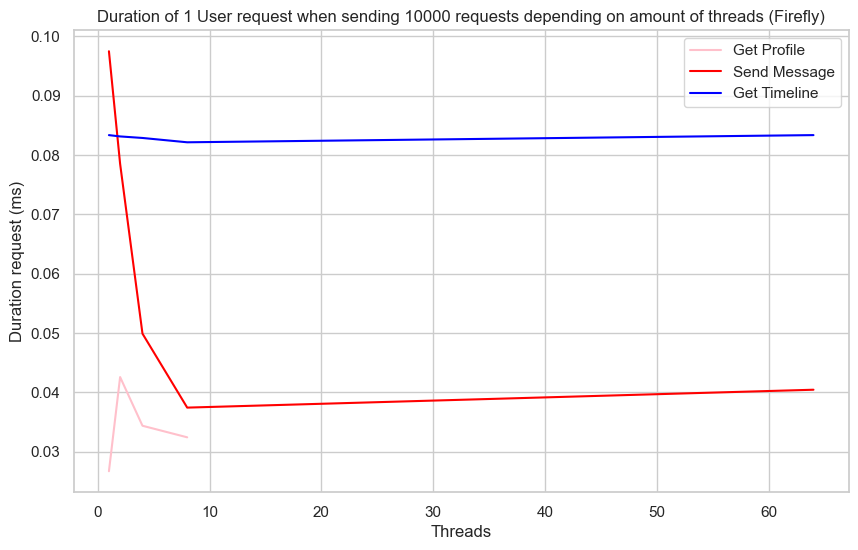
\includegraphics[width = \linewidth]{Images/LatencyFirefly.png}
	\caption{}
\end{figure}
\begin{figure}[H]
	\centering
	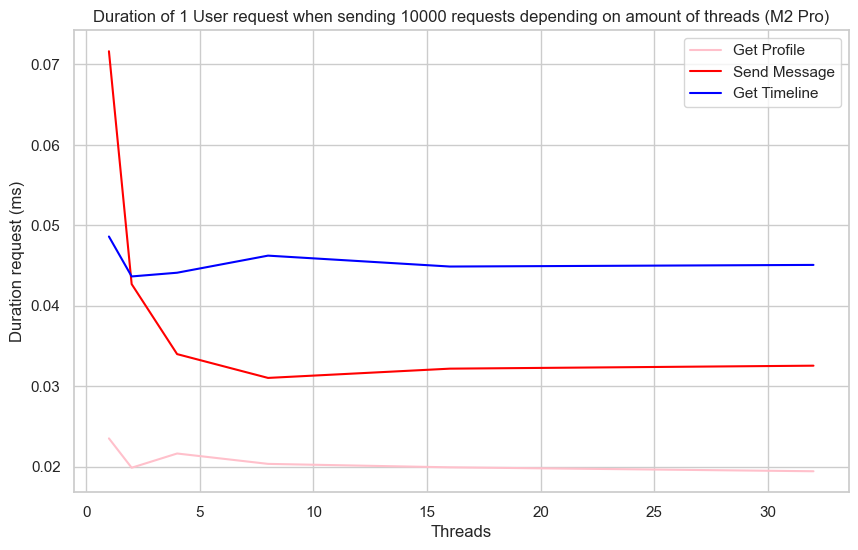
\includegraphics[width = \linewidth]{Images/Latency.png}
	\caption{}
\end{figure}
The latency of sending a message decreases a lot when using multiple threads, this is again because when we send a message, we need to contact a lot of other processes.
When those processes are all on the same thread, we have a bottleneck. Get timeline and get profile have a slight shorter duration of executing when having multiple threads. The latency of getting your profile is overall the best.   


\begin{figure}[H]
	\centering
	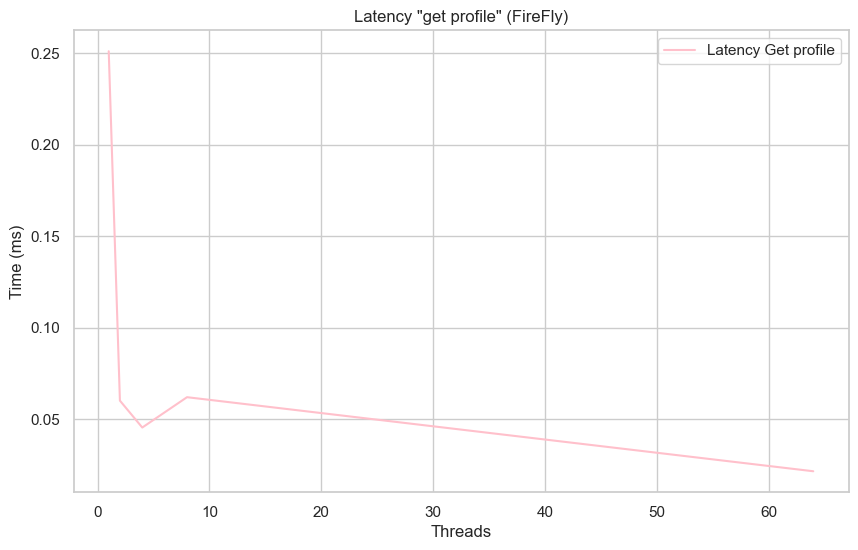
\includegraphics[width = \linewidth]{Images/LatencyProfileFirefly.png}
	\caption{}
\end{figure}
\begin{figure}[H]
	\centering
	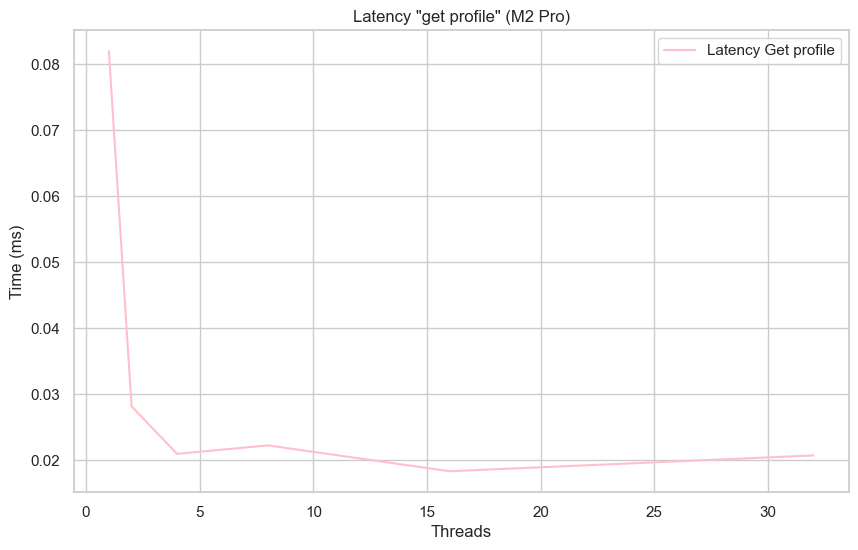
\includegraphics[width = \linewidth]{Images/LatencyProfile.png}
	\caption{}
\end{figure}
When we zoom in on "getting your profile", we also can see a significant difference in duration when having more threads. If you would calcultate the speedup, you would have for 4 threads, and higher, a speedup of 4 (0.08 / 0.02). When we look at Firefly this is even more significant when using more than 4 threads: you would have a speedup of 5 (0.25/0.05). When we look at the speedup of 64 threads, this would have a speedup of 12.5 (0.25/0.02), this is really impressive to see. But keep in mind that we only have 1 benchmark of "get profile" higher with 8 threads for Firefly, so it could be an exception.


Next figures for this experiment will tell us more about the throughput of the different requests. 
\begin{figure}[H]
	\centering
	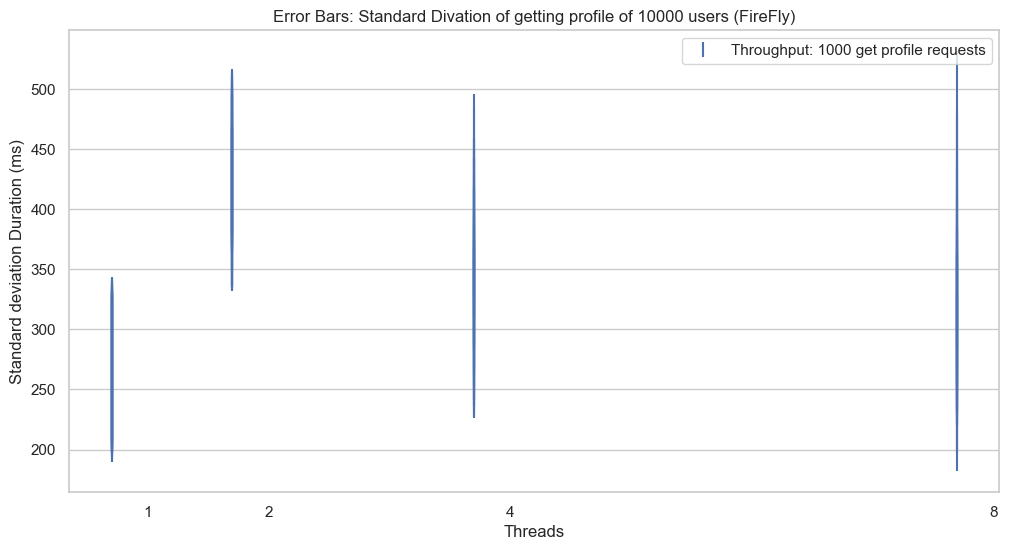
\includegraphics[width = \linewidth]{Images/ThroughputStdFirefly.png}
	\caption{}
\end{figure}
It looks like 4 and 8 threads have some outliers, to make sure this doesn't affect much on the benchmark we will need to make a boxplot to know more where the data is centered.  

\begin{figure}[H]
	\centering
	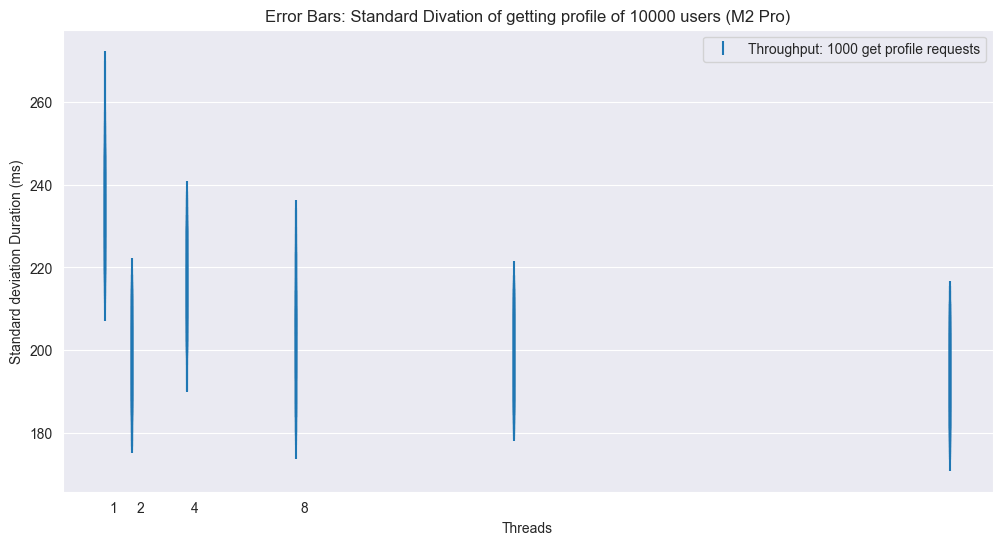
\includegraphics[width = \linewidth]{Images/ThroughputStd.png}
	\caption{}
\end{figure}
Here we can see that when using one thread to get 10000 profiles, the duration is slower than using multiple threads. This is what I expected to happen, but when looking at the data on Firefly this is not really the case, which could have many reasons (other processes, inconsistent actor distribution among the threads, ...). Besides that, I do not see any alarming data.  

\begin{figure}[H]
	\centering
	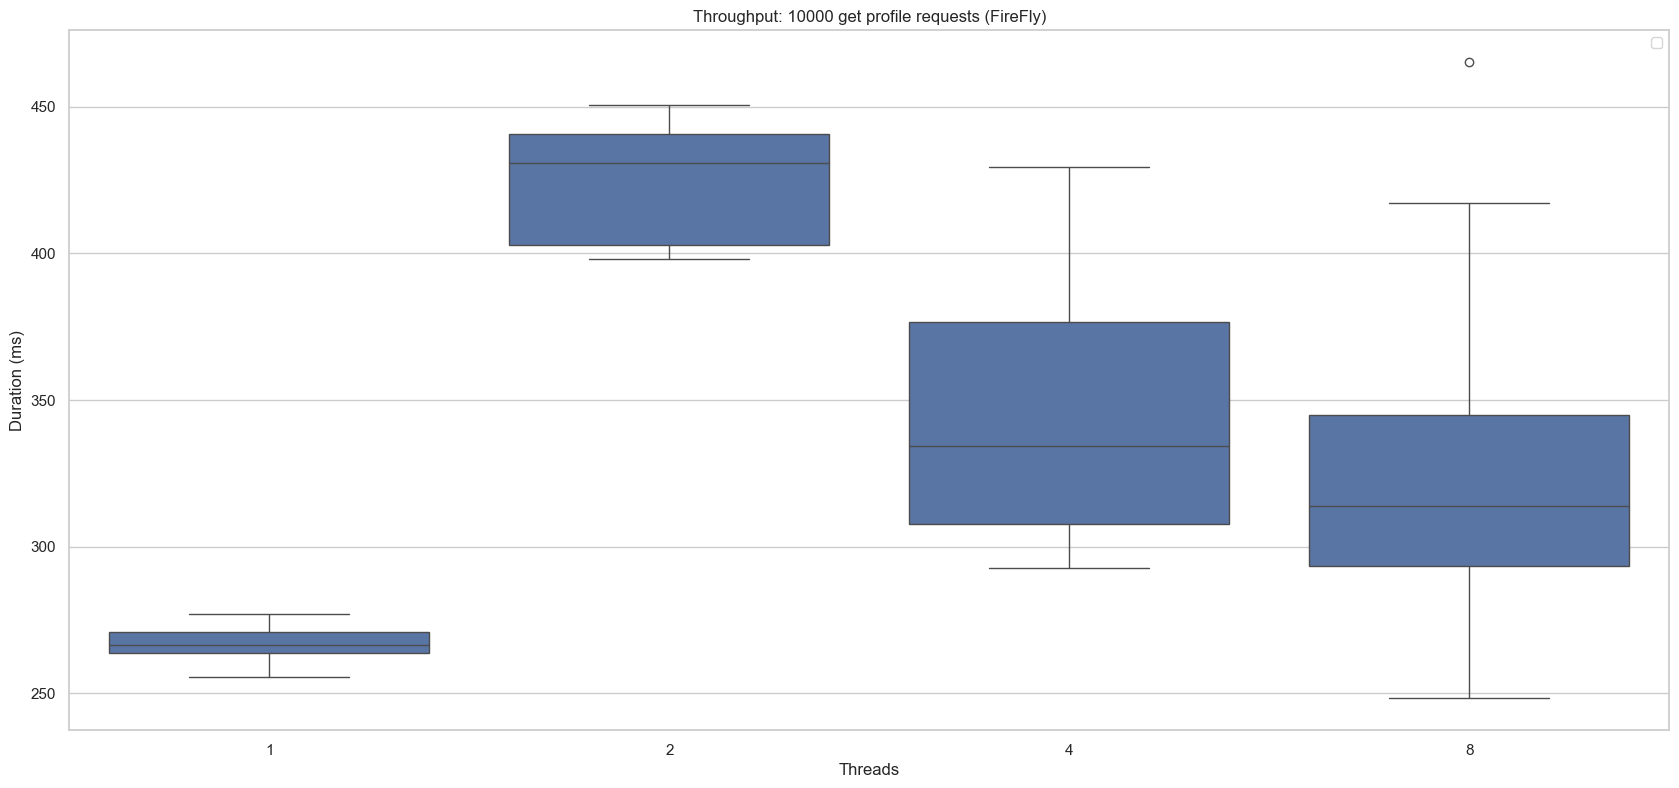
\includegraphics[width = \linewidth]{Images/ThroughputBoxFirefly.png}
	\caption{}
\end{figure}
Here we can see that we have indead some outliers for 4 and 8 threads. This is not alarming because most data is somewhat centered in the box. If the box would be more spread out compared to the other boxes, this would be a bit more alarming. If this was the case, we would need to look more precicly at the data to figure out what happened. 
For the data one thread is very consistent, this can be explained because the chances that the actors are on the same thread is 100\%, the chances that they are on the same thread (when we have 2 threads) is 50\%, and so on. This can explain the outliers when we have more threads, an extra slow datapoint would mean that we send to the user on the same thread, which has a change of 12.5\% for 8 threads).  \\

Confidence level 95\%\\
Confidence Interval 1 Thread: [262.00234259250965, 268.04228240749035]\\
Confidence Interval 2 Threads: [296.45831767697916, 381.3209323230209]\\
Confidence Interval 4 Threads: [419.88430618255853, 436.03119381744153]\\
Confidence Interval 8 Threads: [333.0559131026451, 368.17883689735487]\\

With a confidence level of 95\%, we can say that requesting 10000 profiles will take between x and y time for the correct confidence interval of the number of threads available. If we had done more iterations of the benchmark, our data could have been more consistent, which would 
make more reliable confidence intervals. 
\begin{figure}[H]
	\centering
	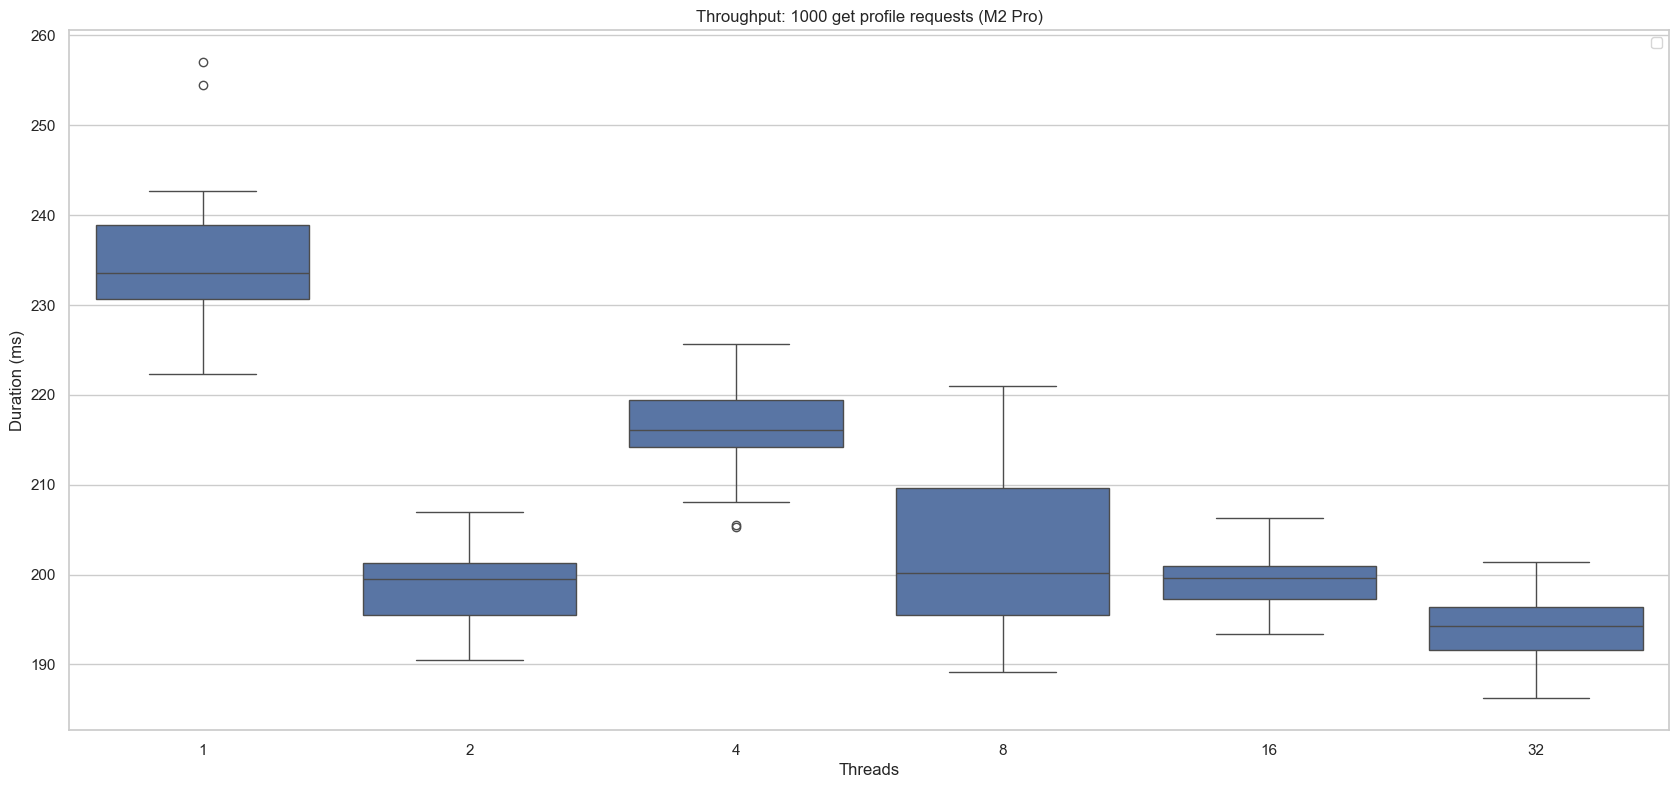
\includegraphics[width = \linewidth]{Images/ThroughputBox.png}
	\caption{}
\end{figure}

Here, we can draw the same conclusions as before. Besides that, we now see that 1 thread is indeed slower than using multiple threads. \\
Confidence level 95\%\\
Confidence Interval 1 Thread: [231.8050380676031, 238.3486419323969] \\
Confidence Interval 2 Threads: [196.8397081109319, 200.3420518890681] \\
Confidence Interval 4 Threads: [214.20028888391275, 218.36915111608724] \\
Confidence Interval 8 Threads: [199.71134022586352, 207.06353977413647] \\

With a confidence level of 95\%, we can say that requesting 10000 profiles will take between x and y time for the correct confidence interval of the number of threads available.


\begin{figure}[H]
	\centering
	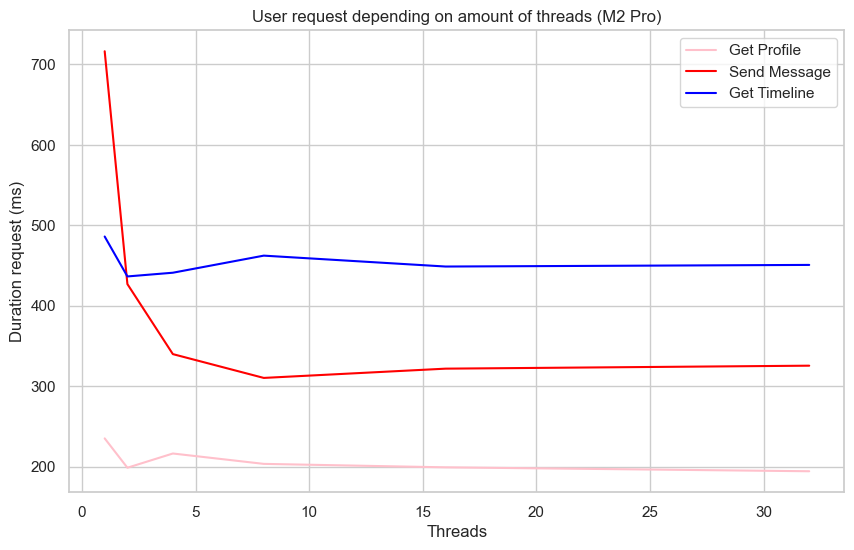
\includegraphics[width = \linewidth]{Images/Throughput.png}
	\caption{}
\end{figure}
We already have seen this figure before, but this also gives us a fast overview of the expected throughput of sending 10000 user request, seperated for get profile, send message and get timeline. Same for the figure of Firefly. For each of these results we could also calcultate the confidence intervals of the different requests a user can execute. Which would gives us a more in depth view. 


\subsubsection{Results Experiment 3}
\begin{figure}[H]
	\centering
	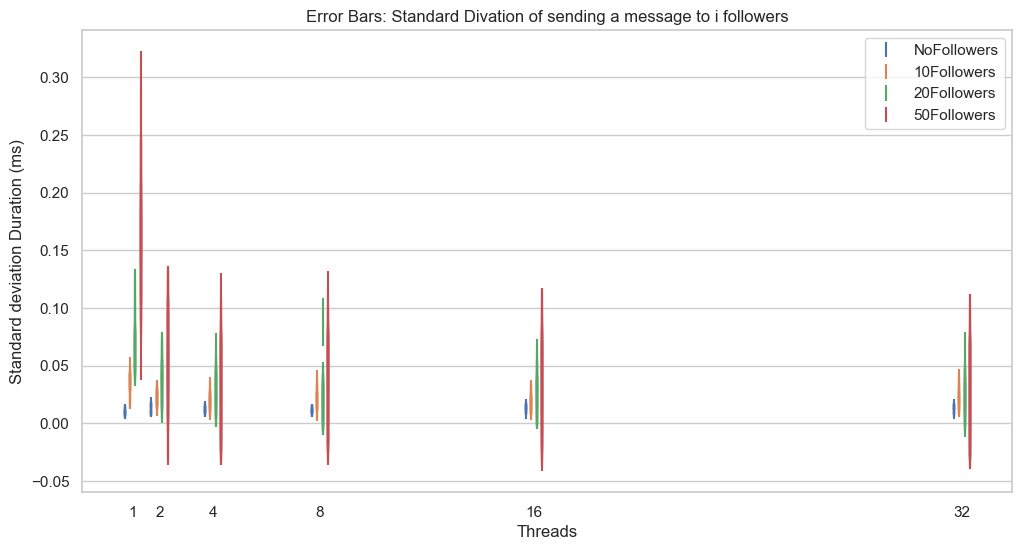
\includegraphics[width = \linewidth]{Images/ErrorBarsLatency.png}
	\caption{}
\end{figure}
\begin{figure}[H]
	\centering
	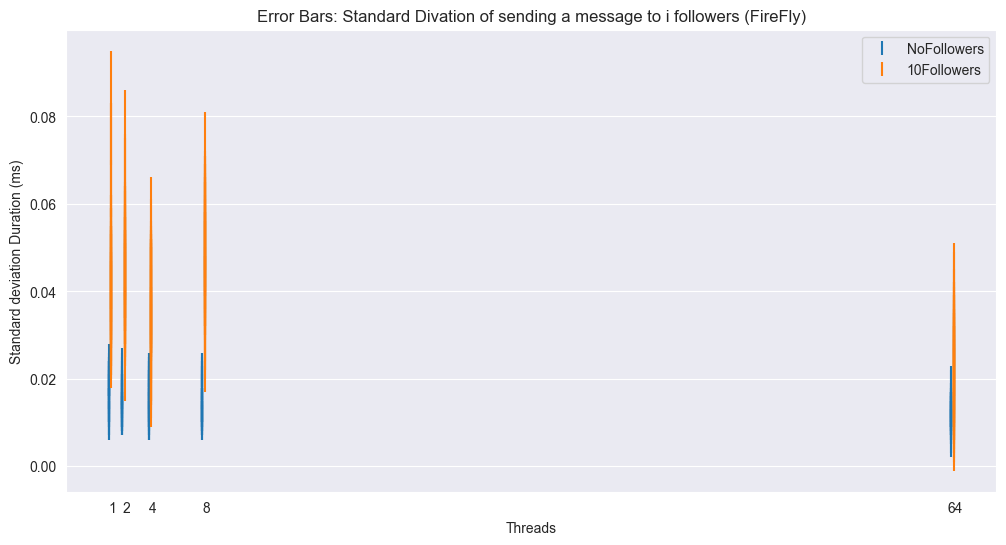
\includegraphics[width = \linewidth]{Images/ErrorBarsLatencyFireFly.png}
	\caption{}
\end{figure}
Out of the figures above, we can see that how more followers a user has, how longer the request can take, how greater the standard deviation is. These are not really alarming error points that need further investigation. 
\begin{figure}[H]
	\centering
	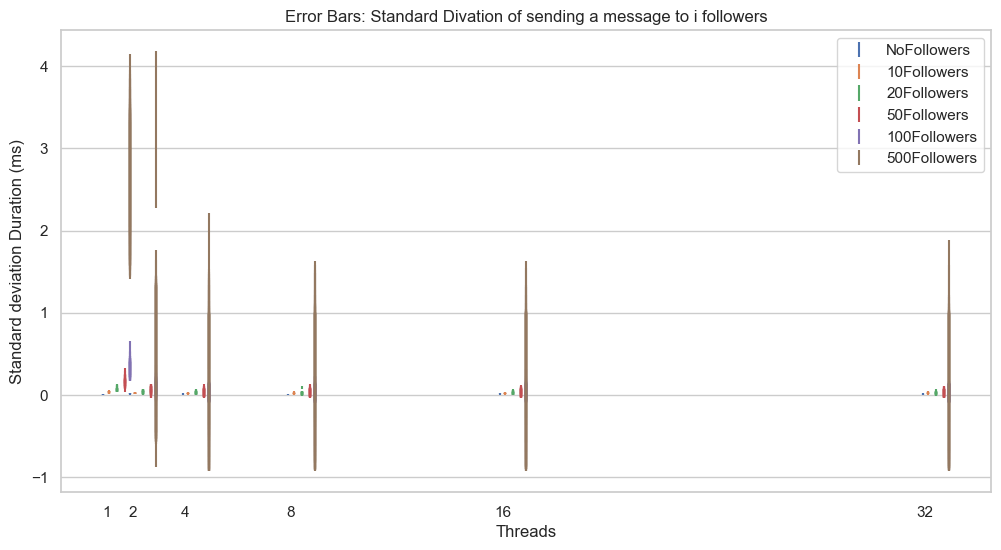
\includegraphics[width = \linewidth]{Images/ErrorBarsLatencyFull.png}
	\caption{}
\end{figure}
Here is an extra figure for the data of 100 followers and 500 followers, I chose to make this a seperate figure because sending to 500 different actors was way more time consuming than sending to a lower number of users, so our conclusion of previous graphs would be less clear. But for showing that I tested it for 100 and 500 followers, I displayed it in the figure above. 

\begin{figure}[H]
	\centering
	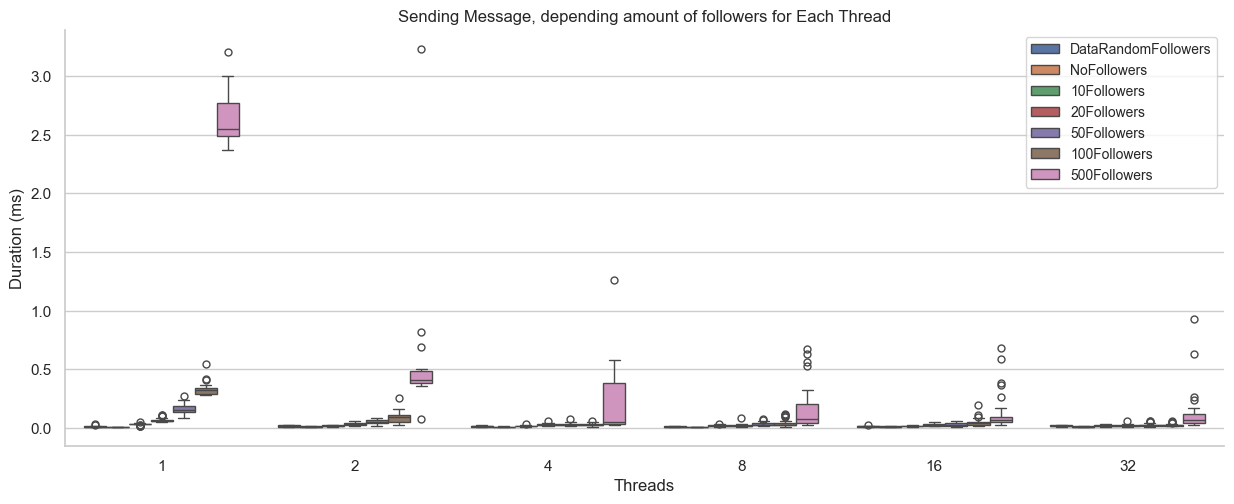
\includegraphics[width = \linewidth]{Images/SendingMessageLatencyBox.png}
	\caption{}
\end{figure}
In the boxplot we can make the same conclusions as before, but here we can also see that 500 followers will have more outliers that are further away from the boxplot. But here we can see that the size of the boxplot of 500 users becomes smaller when having more threads. And the boxplot shrinks in a more preferable duration of the request. Out of this, parallelising many actors that communicate a lot with each other is beneficial. 
\begin{figure}[H]
	\centering
	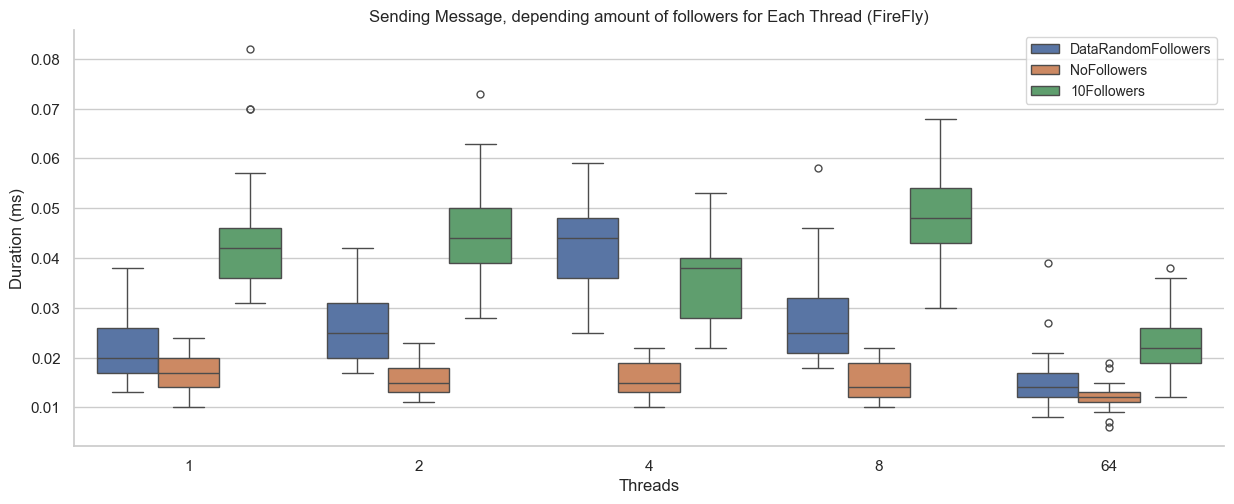
\includegraphics[width = \linewidth]{Images/SendingMessageLatencyBoxFireFly.png}
	\caption{}
\end{figure}
Here again we can see, for 64 threads, that the boxplot becomes smaller and better in duration of the request, even for smaller amounts of communications. We also saw this in the speedup of sending a message from experiment 1. When having no followers, there is a less significant difference because we don't need to contact other actors that are possibly on different threads. This request is thus primarily sequential. We can also see that, how more followers a person has, how longer it takes to process a send message request. In following boxplots we can seperatly see how long it takes to broadcast a message to 10, 20, 50, 100 and 500 users. So the time that the first user sees the message in the timeline will be faster then when it arrives by the last users. Of course, in real circumstances, we have distributed systems for this cause, and the time of arrival also differs from other factors (ex, distance that a message needs to cover).  

\begin{figure}[H]
	\centering
	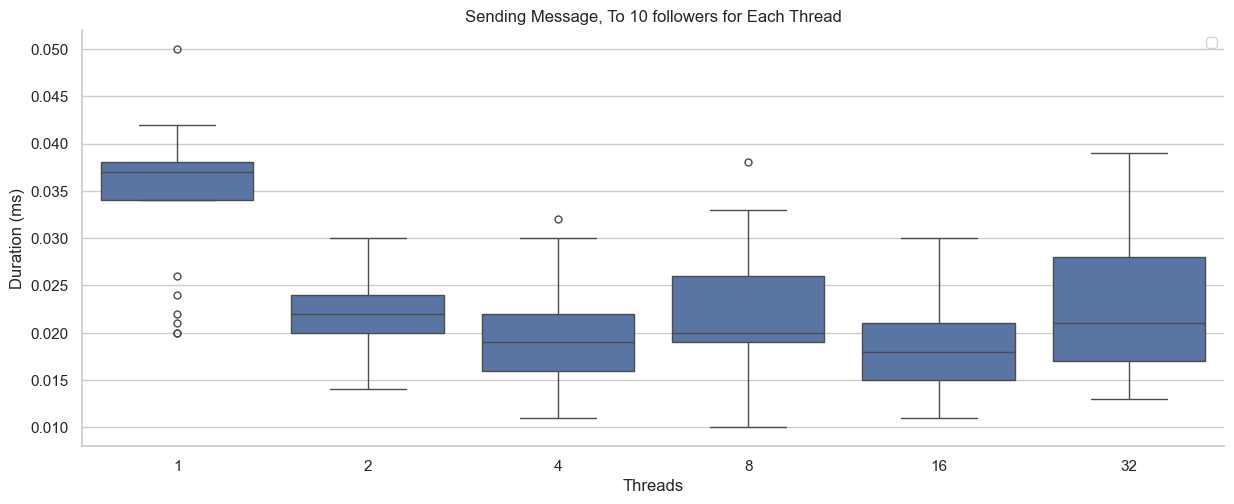
\includegraphics[width = \linewidth]{Images/SendingMessageBox10Follower.png}
	\caption{M2 pro}
\end{figure}

\begin{figure}[H]
	\centering
	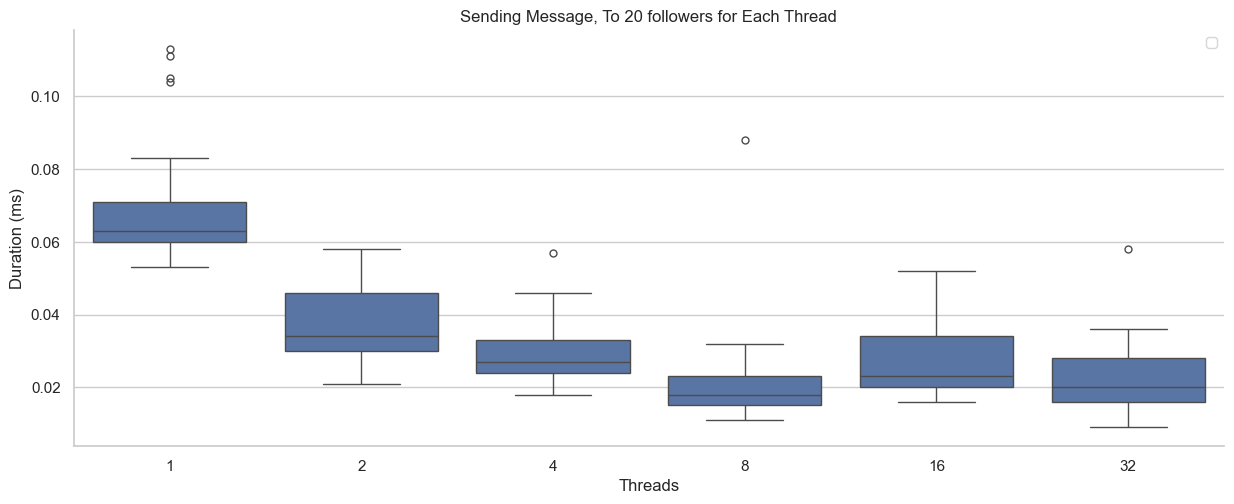
\includegraphics[width = \linewidth]{Images/SendingMessageBox20Follower.png}
	\caption{M2 pro}
\end{figure}

\begin{figure}[H]
	\centering
	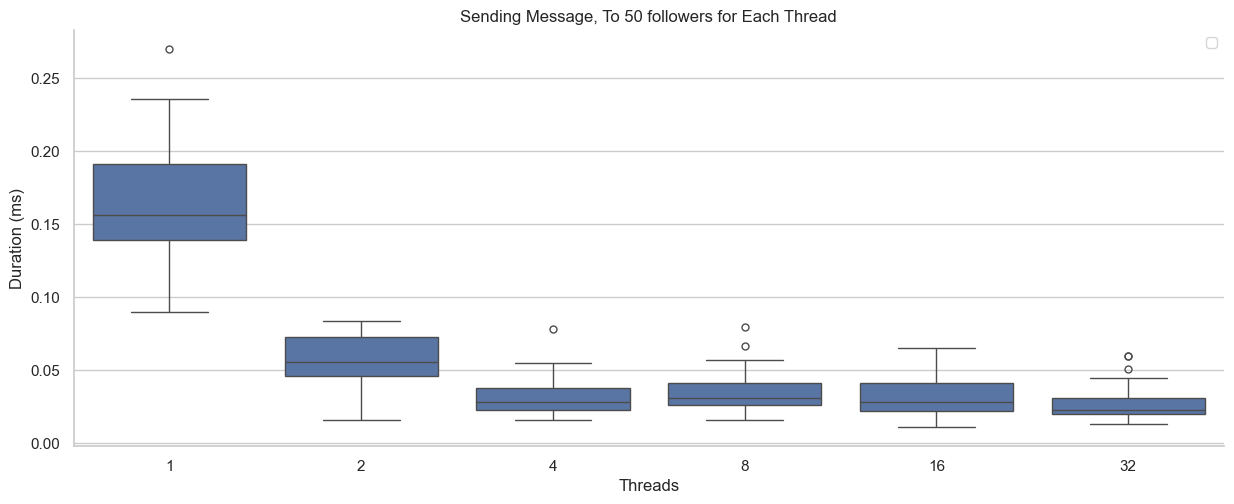
\includegraphics[width = \linewidth]{Images/SendingMessageBox50Followers.png}
	\caption{M2 pro}
\end{figure}
\begin{figure}[H]
	\centering
	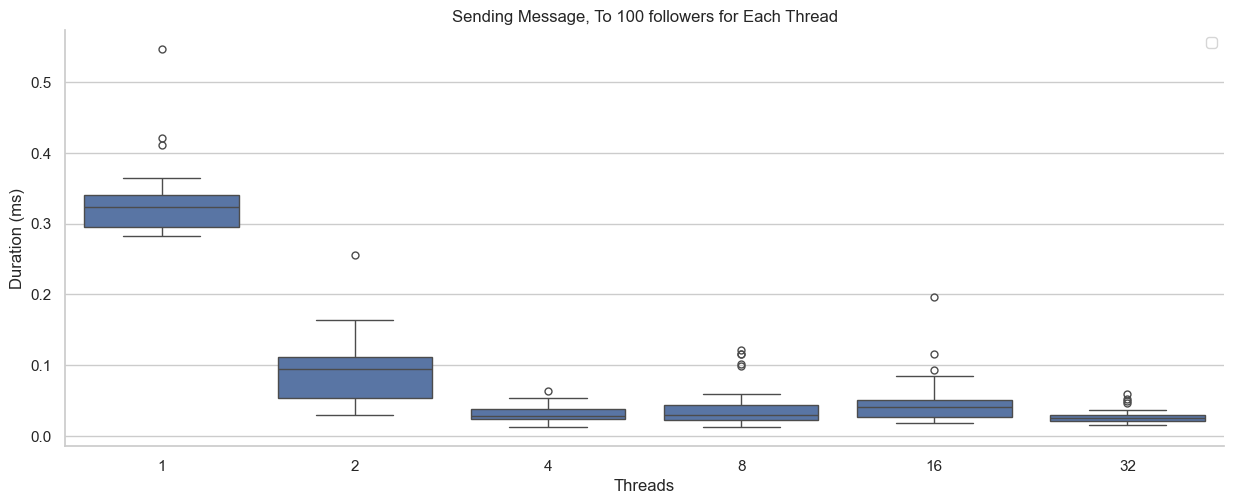
\includegraphics[width = \linewidth]{Images/SendingMessageBox100Follower.png}
	\caption{M2 pro}
\end{figure}
\begin{figure}[H]
	\centering
	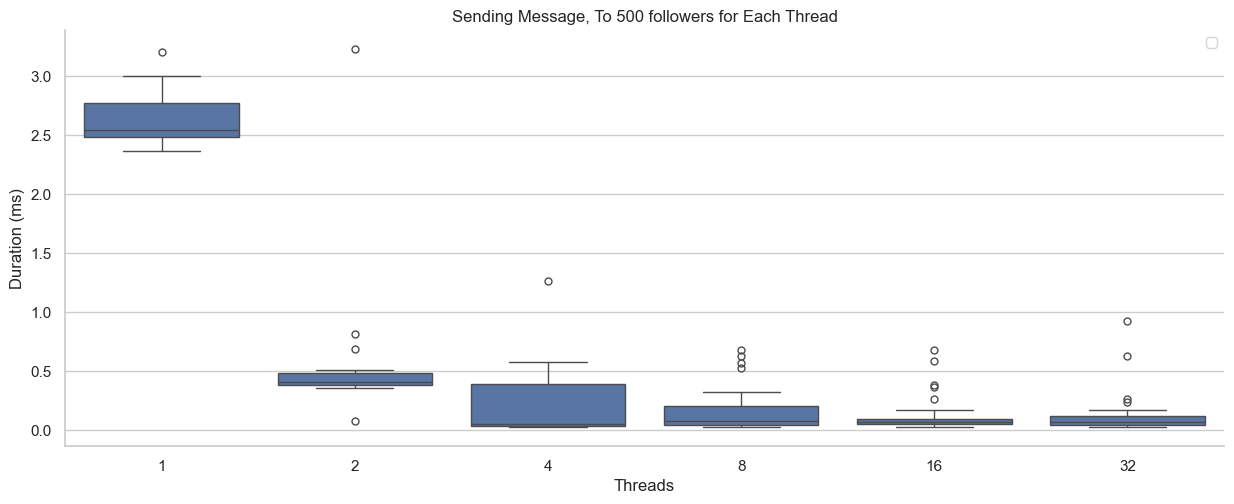
\includegraphics[width = \linewidth]{Images/SendingMessageBox500Follower.png}
	\caption{M2 pro}
\end{figure}

\begin{figure}[H]
	\centering
	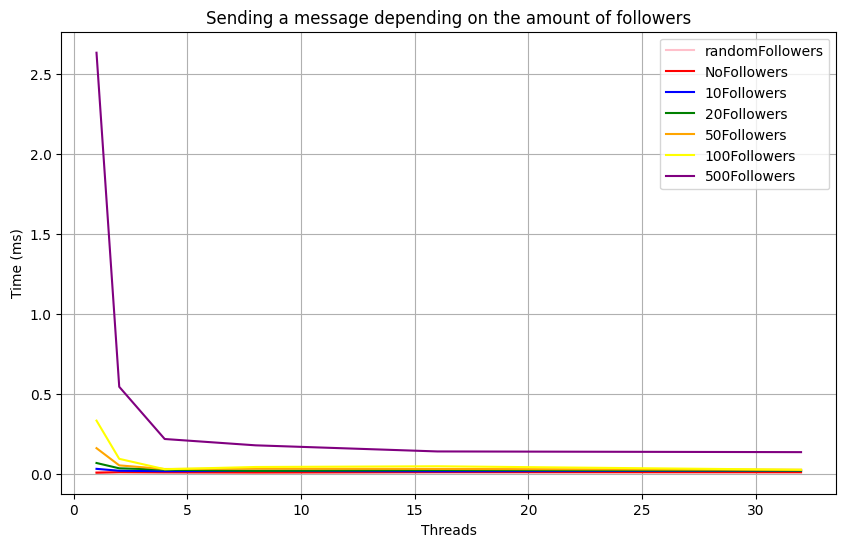
\includegraphics[width = \linewidth]{Images/SendingMessageLatencyMean.png}
	\caption{M2 pro}
\end{figure}
In the above figure we can see how long it takes to send messages to x amount of actors, on y amount of threads. We can see that when using 1 thread, and change the amount of actors to reach, the difference is more pronounced then when parallelizing the data.  
\begin{figure}[H]
	\centering
	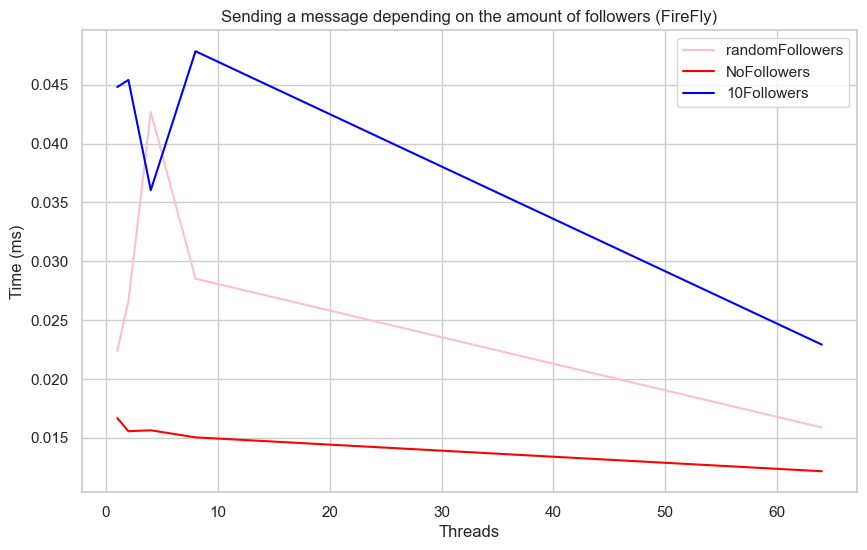
\includegraphics[width = \linewidth]{Images/SendingMessageLatencyMeanFireFly.png}
	\caption{FireFly}
\end{figure}


\begin{figure}[H]
	\centering
	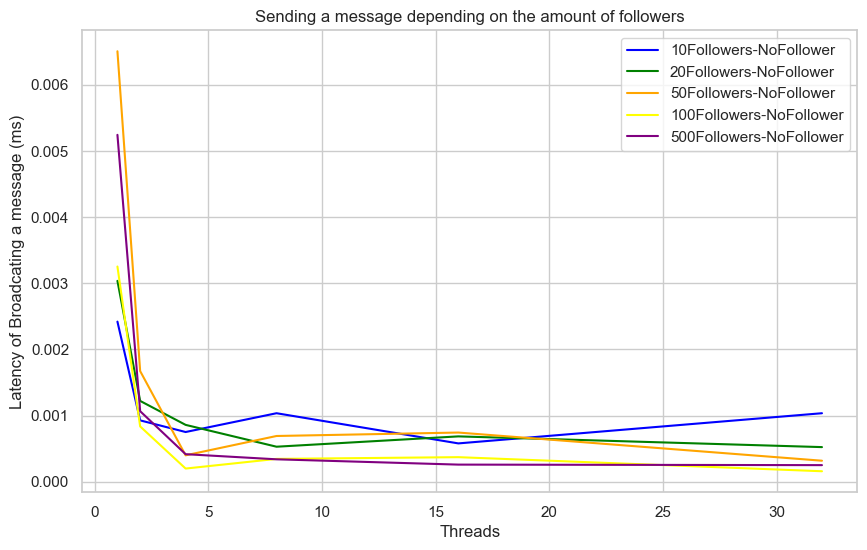
\includegraphics[width = \linewidth]{Images/SendingMessageLatency-Mean.png}
	\caption{M2 Pro}
\end{figure}
The time in the y-axis tells us how long it would take to contact 1 actor. \\


In the 2 above figures, you can see the time it takes to send to 1 actor, depending on how many requests are sent to different actors. When contacting 500 actors, it is more likely that we sometimes contact the same actor, or actors on the same thread. This is why the latency is higher when having more followers. But when we parallelise it more and more we see that the lines cross each other and it doesn't matter as much anymore how much followers you have. Here we can cleary see that the speedup of more requests would have a higher speedup.  


\section{Insight Question}

\subsubsection{spawning a process in Erlang is a very lightweight operation: a newly spawned Erlang process only uses 309 words of memory. How has this influenced your solution? Imagine the cost of
creating a process was much higher, e.g. if you were using Java and created new Threads: how
would this affect the performance and how could you improve this?
}

If we would use a program that has more higher weigth processes, then making too many tasks depending on the amount of threads would give us an overhead of the implementation. If we would have higher cost processes, I could change my threshold depending on the amount of processors available on the system. If we do not know how much processors there are available, we could benchmark and out of the benchmarks we could conclude which threshold would fit the overall implementation the best. Having the benefit of lightweigth processes in Erlang, reflected on the fact that having 1 user/actor performed the best. If our processes where more costly we wouldn't benefit from having only 1 user per process. 

\subsubsection{Twitter and Threads provide two types of homepage: "Following" and "For You". The page "Following" contains the timeline as we implemented it, consisting of a chronological list of messages from the users you follow. The page "For You" contains a list of messages that are gathered both from users you follow as well as other "popular" messages on the platform,
and are then sorted using a machine learning algorithm. How would you implement this in
your system? Do not focus on the machine learning algorithm, but discuss the impact on the
architecture and performance of your system.} 
I think getting the "following page" is pretty well defined in my implementation because I focussed on making the timeline as performant as possible (which has a negative effect on data duplication), but I would only save a certain time period, and delete the older messages to have less duplicated data in the long run and fetch them whenever a user has fully scrolled down its timeline). But for the for you page, I would get the best-rated posts in my timeline (which should be easy to get). And for the popular messages from "non following", I would make actors for person groups (for ex, people who like footbal and between a certain age, teenagers that like skin and haircare, ...) and then contact the correct actors depending on the users interest to get popular new messages to then merge with the popular timeline messages. 


%\bibliography{bibliography}
\end{document}
